% LaTeX2e Template by Stephen Iota (https://stepheniota.github.io/)
% last updated: Oct. 2018

% for papers
%\documentclass[aps,onecolumn,superscriptaddress]{revtex4-1}
% https://www-d0.fnal.gov/Run2Physics/WWW/templates/revtex4.pdf
% https://cdn.journals.aps.org/files/revtex/auguide4-1.pdf
% for revTeX4-1 class options

% for other
\documentclass[11pt]{article}
\usepackage[margin=2cm]{geometry}

%%%%%%%%%%%%%%%%
%%% Packages %%%
%%%%%%%%%%%%%%%%

\usepackage[utf8]{inputenc}
\usepackage{amsmath}
\usepackage{amssymb}
\usepackage{amsfonts} % to remove math font when typesetting equations
\usepackage{graphicx}
\usepackage{enumitem} % to change labels in enum/item
\usepackage[dvipsnames]{xcolor} % for colored links


% always put this at the end
\usepackage[
	colorlinks=true,
	citecolor=green!50!black,
	linkcolor=NavyBlue!75!black,
	urlcolor=green!50!black,
	hypertexnames=false]{hyperref} 

 
 %%%%%%%%%%%%%%%%%%
 %% New Commands %%
 %%%%%%%%%%%%%%%%%%
 
\newcommand{\email}[1]{\texttt{\href{mailto:#1}{#1}}}

\newcommand{\hint}[1]{\color{Blue}{#1}}
 
%----------------------------------------------------
%%%%%%%%%%%%%%%%%%
%% Front Matter %%
%%%%%%%%%%%%%%%%%%

\pagenumbering{gobble} % no page numbers
\graphicspath{{figures/}} % set directory for figures


%%%%%%%%%%%%%
%%% Title %%%
%%%%%%%%%%%%%
\begin{document}

\begin{center}

\Large{\textsc{Worksheet 2b}: \textbf{Gauss's Theorem}}

\end{center}

\vspace{.5mm}

%%%%%%%%%%
%% INFO %%
%%%%%%%%%%

\begin{tabular}{rl}
\textsc{SI Leader}:
&
Stephen Iota (\email{siota001@ucr.edu})
\\
\textsc{Course}:
&
Physics 40C (Fall 2018), Dr.~Laura Sales
\\
\textsc{Date}:
&
11 October 2018
\end{tabular}

%%%%%%%%%%%%%%
%% PROBLEMS %%
%%%%%%%%%%%%%%


\section{Conceptual Questions}

\begin{enumerate}[label=(\alph*)]

\item A metallic sphere of radius $r = 5 \ \mu$m with a total charge of $-12.3$ nC is placed in an electric field $\vec{E}(\vec{r}) = 3.2 \hat{x} + 5.7 \hat{y}  - 7.3 \hat{z}$ N/C. What is the electric field strength inside ($r<R$) the sphere?
\item Is Gauss's Law only valid for symmetric charge distributions?  	

\end{enumerate}

 
\section{What the Flux}

\begin{enumerate}[label=(\alph*)]

\item What is the net electric flux through the cylinder below?
\begin{center}
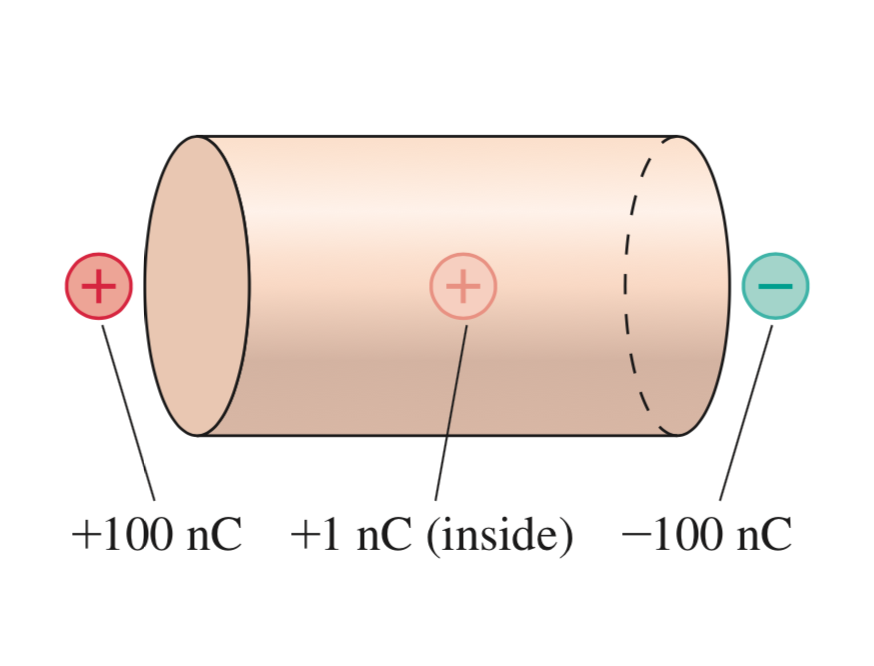
\includegraphics[width=.3\linewidth]{W2b_fig2}
\end{center}
\item What is the surface area of a sphere? What is the volume of a sphere?

\item For a symmetric sphere, prove:
$$\Phi_{e} = \oint_{S} \vec{E} \cdot \mathrm{d}\vec{A} = E\cdot4\pi r^2$$ 
	
\end{enumerate}

\section{Cylindrical Symmetry}
\begin{center}
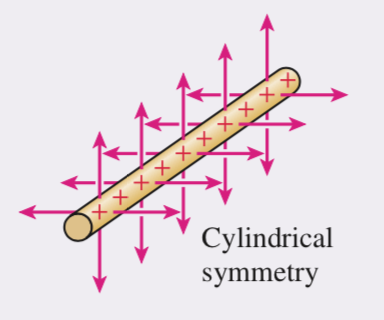
\includegraphics[width=.3\linewidth]{W2b_fig1}
\end{center}
\begin{enumerate}[label=(\alph*)]
	\item What is the surface area of the rod of length $L$?
	\item The net electric flux coming out through the cylinder is $-1000$ Nm$^2$/C. How much charge is enclosed   within the cylinder?
\end{enumerate}


\end{document}